% Template for ICASSP-2016 paper; to be used with:
%          spconf.sty  - ICASSP/ICIP LaTeX style file, and
%          IEEEbib.bst - IEEE bibliography style file.
% --------------------------------------------------------------------------
\documentclass{article}
\usepackage{spconf,amsmath,graphicx,float}

% Example definitions.
% --------------------
\def\x{{\mathbf x}}
\def\L{{\cal L}}

% Title.
% ------
\title{Automated Landmark Recognition Powered by Deep Learning}
%
% Single address.
% ---------------
\name{Jifu Zhao}
%\address{Department of Nuclear, Plasma, and Radiological Engineering \\
%University of Illinois at Urbana-Champaign, Urbana, Illinois 61801, USA}

\address{University of Illinois at Urbana-Champaign, Urbana, Illinois 61801, USA}

\begin{document}
%\ninept
%
\maketitle

% --------------------------------------
\section{Introduction}
\label{sec:intro}
With the development of deep learning techniques, especially convolutional neural networks (CNN), people have achieved huge breakthrough on computer vision in recent years. For example, on ImageNet Large Scale Visual Recognition Challenge, computer have achieved human-level error rate. Some classical CNN models, such as VGG, ResNet, and Inception, have been widely adapted to various computer vision tasks. 

One important factor that contributes to the success of image object recognition is the large number of training images. For example, CIFAR-10 dataset contains of 60,000 color images in 10 classes, with 6,000 images per class, and ImageNet dataset contains of 1,000 objects. In addition to similar problems with large amount of training images, there are problems without large amount of training set or the number of objects is too large such that some objects only have a small number of or even one images in training set, which make it impossible to apply the same supervised algorithms. Problems like face recognition, landmark recognition and so on, are very challenging due to small number of training images for each object. This work, using a recently released landmark dataset from Google, try to explore the application of deep learning methods on landmark recognition problems.

% --------------------------------------
\section{Problems}
\label{sec:problem}
Problems such as face recognition and landmark recognition can be categorized as one shot learning problem. For this kind of problems, for each object, there might be only a limited number of images. For example, for a face recognition, it is pretty common that each person only have several or even one images in the training set. In addition, there could be a lot of objects to be recognized. For example, a face recognition system may need to correctly identify thousands of person. This kind of problems is pretty challenging even now. Fig.~\ref{fig:example} shows a typical scenario of landmark recognition.

\begin{figure}[htbp]
\centering
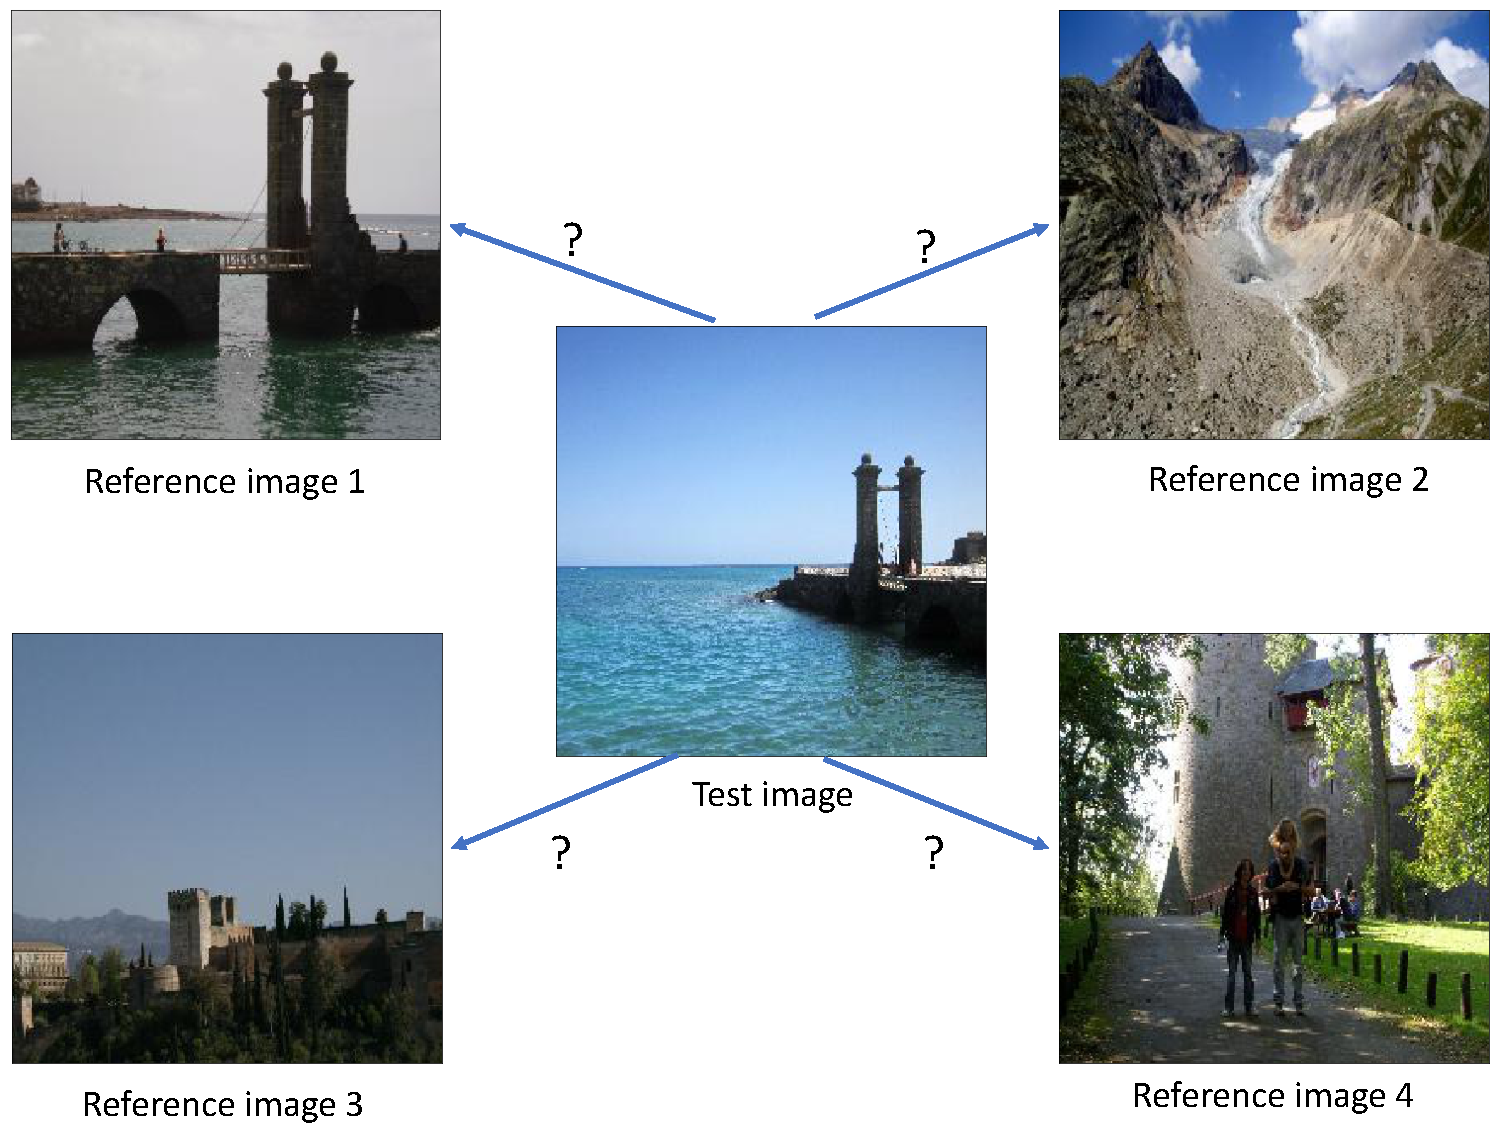
\includegraphics[width=7.0cm]{./figures/sample.pdf}
\caption{Illustration of landmark recognition problem.}
\label{fig:example}
\end{figure}

% --------------------------------------
\section{Dataset}
\label{sec:dataset}
Recently, Google released a large landmark dataset on Kaggle. It contains more than 1 million images labelled into 14,951 different landmarks. Some famous landmarks contains a huge number of training images. However, for the not-so-famous landmarks, there is less labelled images. The large number of classes and few number of training examples per class increase the complexity of the problem.

The given dataset only contains the url and landmark id for each image. All the images need to be downloaded from online and different images have different size and resolution. The large number of training images, preprocessing steps, and the large number of images to analyze, make this problem challenging for both algorithms and computation power.


% --------------------------------------
\section{Summary}
\label{sec:summary}

The goal of this project is to explore the application of deep learning for landmark recognition problems. Currently, the tentative plans include: using pretrained CNN models such as VGG19, ResNet, and Inception to extract the abstract features for each images. Through this step, the dimensionality of the training set is dramatically reduced, and the original images are represented using more meaningful features. With the extracted features, next step is to learn function that can correctly identify the correct label for each images. Siamese neural networks and Triplet loss learning, for example, might be appropriate for similar problems.

To summarize, this work try to apply deep learning techniques on real-world large-scale dataset to gain some insights one landmark recognition problems. Due to the large amount of images, limited computation power, and unpredicted difficulties, the final result might not be as good as expected.


%\begin{figure}[htbp]
%\centering
%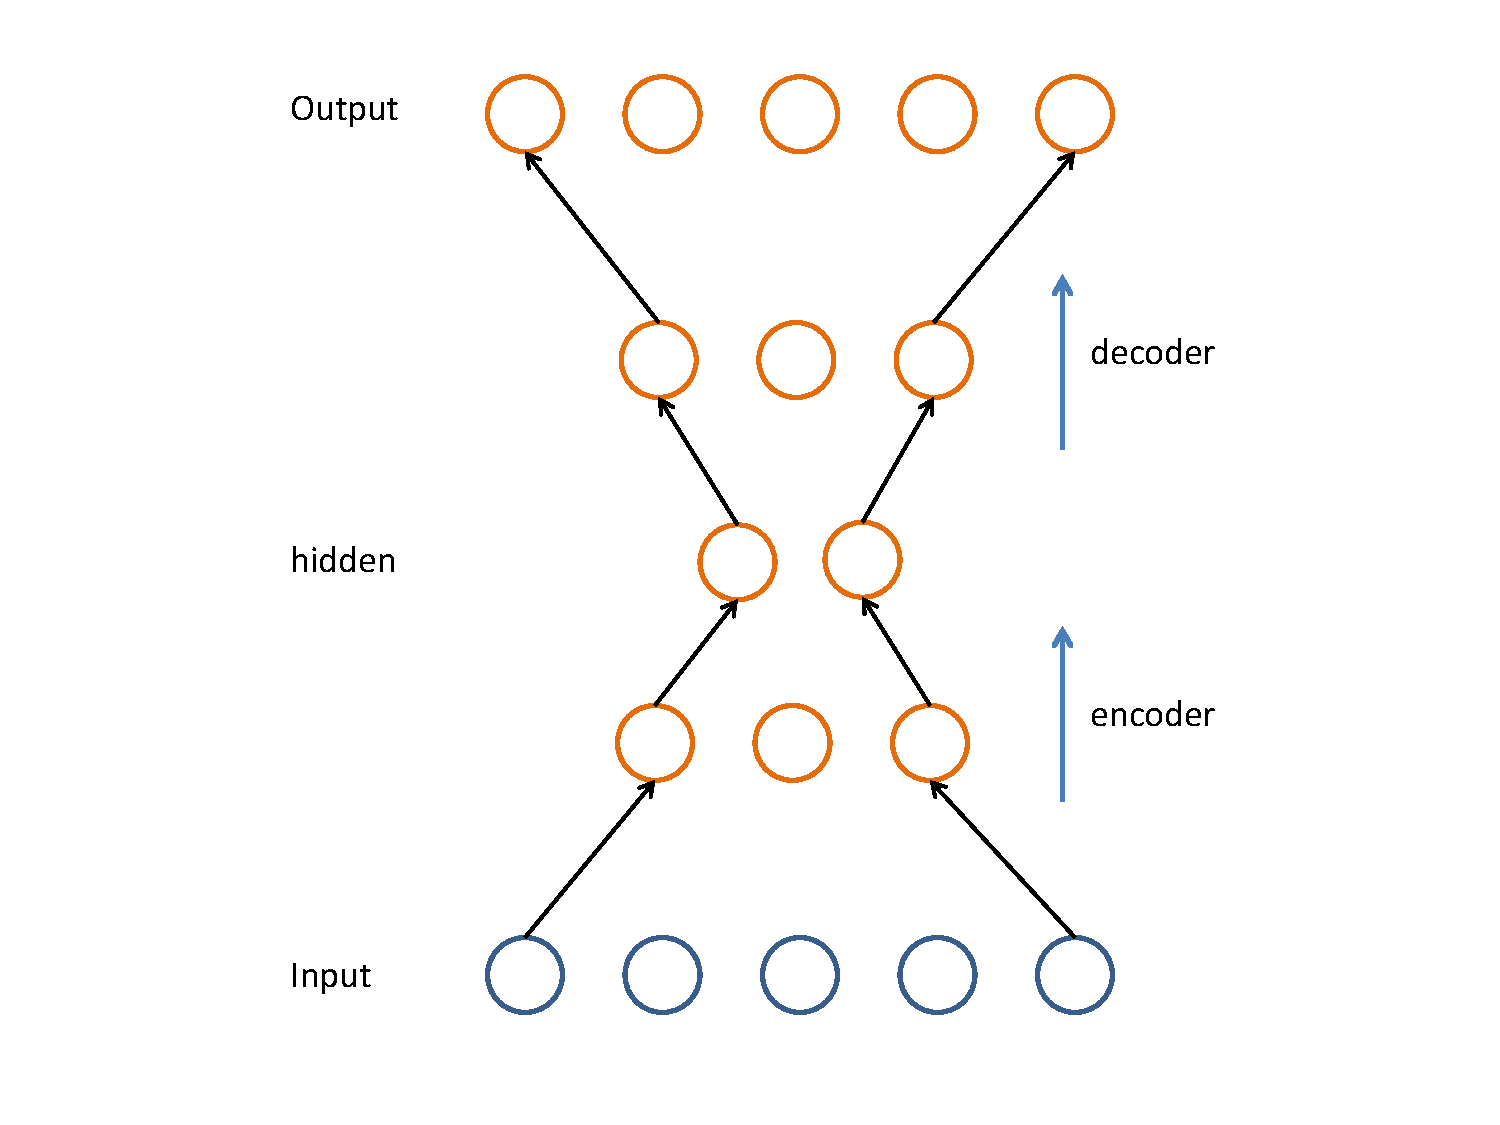
\includegraphics[width=8.5cm]{./figures/autoencoder.pdf}
%\caption{Illustration of auto-encoder system.}
%\label{fig:autoencoder}
%\end{figure}

\vfill\pagebreak

% References should be produced using the bibtex program from suitable
% BiBTeX files (here: strings, refs, manuals). The IEEEbib.bst bibliography
% style file from IEEE produces unsorted bibliography list.
% -------------------------------------------------------------------------
\bibliographystyle{IEEEbib}
%\bibliography{strings,refs}
\bibliography{strings}

\end{document}
